%% plainproblemname: Fiskspelet
\problemname{Fiskspelet}
Du spelar fiskspelet. Du är en fisk som ska äta mindre fiskar men aldrig får
bli uppäten av större fiskar. Fiskarna ändrar aldrig storlek. Du får poäng för varje fisk du äter och självklart vill du ha så mycket
poäng som möjligt.

Spelplanen kan ses som ett rutnät med $H$ rader (numrerade från 1 till $H$) men obegränsat antal kolumner. Du befinner dig i kolumnen $x=0$ och kan bara röra dig vertikalt (uppåt och nedåt). De andra fiskarna rör sig däremot aldrig vertikalt utan börjar i en viss kolumn $x>0$ och flyter med konstant fart åt vänster (mot din kolumn). 

Alla fiskar (även du) har bredden 1 ruta. Din höjd är 7. Det finns tre andra sorters fiskar: ``liten'' med höjd 3, ``mellan'' med höjd 5 och ``stor'' med höjd 9. Fiskarna har olika hastigheter. Varje sekund kan du röra dig en ruta uppåt eller nedåt (eller stå stilla). På samma tid rör sig en liten fisk 1 ruta, en mellanfisk 2 rutor och en stor fisk 3 rutor åt vänster. Du väljer själv på vilken höjd-nivå din fisk ska börja, men observera att \emph{hela} fisken alltid måste vara inom spelplanen. 
%Det innebär att din mittenruta alltid måste vara inom intervallet $[4, h-3]$. THIS INFO IS NOT NEEDED I THINK


En fisk kan äta fiskar som är mindre än den själv. Du kan alltså äta fiskar av storlek 3 och 5, och får då 10 respektive 20 poäng. Men fiskar av höjd 9 kommer att äta upp dig, och du måste akta dig för dem. Skulle du bli uppäten förlorar du. För att det inte ska bli orättvist vem som
äter vem så har sjöjungfrun Arashiel bestämt att följande sker i varje diskret
sekundsteg:
\begin{enumerate}
  \item
     Du gör ditt drag (flyttar upp, ner, eller stannar kvar).
  \item
     Stora fiskar avancerar tre steg, mellan-fiskar avancerar två steg och små fiskar avancerar ett steg.
  \item
     Stora fiskar äter mellan- och småfiskar (eller dig) om de är i samma kolumn och överlappar vertikalt (minst en ruta gemensam).
  \item
     Mellanfiskar som överlevt äter småfiskar om de är i samma kolumn och överlappar vertikalt.
  \item
     Du äter små- och mellanfiskar om de är i din kolumn ($x=0$) och överlappar vertikalt.
\end{enumerate}

\section*{Indata}

På första raden står två heltal, $N$ ($1 \leq N \leq 50\,000$), antalet fiskar, och $H$ ($20 \leq H \leq 1\,000$), höjden på banan. Sedan följer $N$ rader,
en för varje fisk. På varje rad står först en bokstav, \texttt{L}/\texttt{M}/\texttt{S}, alltså om fisken är liten, mellan eller stor. Därefter följer kolumnen $x$ som fisken startar på ($2 \leq x \leq 10^{16}$), samt vilken rad $y$ som utgör fiskens mellersta ruta (alltid vald så att hela fisken får plats inom intervallet $[1, h]$). De tre värdena åtskiljs med blanksteg.

Dessutom gäller att:
\begin{itemize}
  \item
    Inga fiskar i indata kommer överlappa varken helt eller delvis (initialt).
  \item
      $x$-koordinaten för varje fisk kommer alltid att vara jämn. För den större
      fiskstorleken kommer den även alltid att vara delbar med 3. Detta
      eftersom vi vill att alla krockar ska ske på heltalskoordinater.
  \item
    Du kommer alltid kunna klara dig från att bli uppäten, dvs spelet har
    alltid en lösning.
\end{itemize}

\section*{Utdata}
Skriv ut en rad med ett enda heltal, antalet poäng du får om du spelar spelet optimalt.

\section*{Poängsättning}
Din lösning kommer att testas på en mängd testfallsgrupper.
För att få poäng för en grupp så måste du klara alla testfall i gruppen.

\noindent
\begin{tabular}{| l | l | l |}
  \hline
  Grupp & Poängvärde & Gränser \\ \hline
  $1$   & $20$       & $N \leq 1000$, $H \leq 50$, $x \leq 10\,000$ \\ \hline
  $2$   & $20$       & $H \leq 50$, inga fiskar äter upp varandra \\ \hline
  $3$   & $20$       & $H \leq 50$, mellanfiskar äter aldrig småfiskar \\ \hline
  $4$   & $20$       & $H \leq 50$ \\ \hline
  $5$   & $20$       & Inga ytterligare begränsningar \\ \hline
\end{tabular}

\section*{Förklaring av exempelfall}
\begin{figure}[h!]
    \centering
    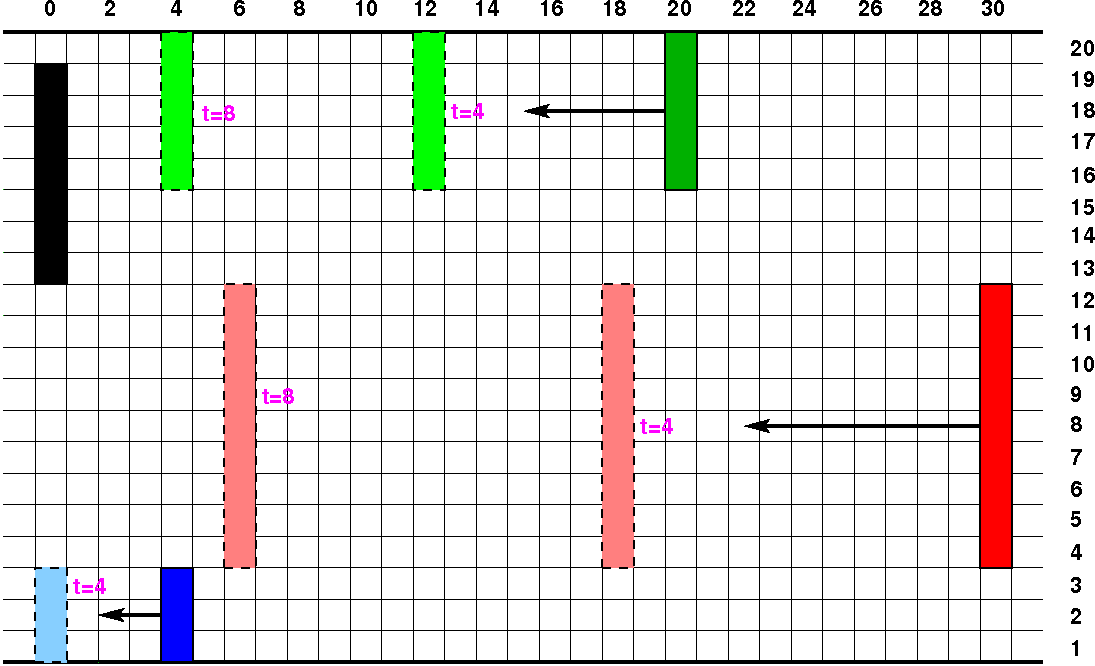
\includegraphics[width=0.75\textwidth]{fiskspelet.png}\\
\caption{Situationen i exempelfall 1}
\label{fig:sample1}
\end{figure}
En möjlig lösning till det första exemplet visas i figur~\ref{fig:sample1}.
De heldragna färgade rektanglarna
visar fiskarnas utgångspositioner och de streckade rektanglarna visar
deras positioner efter $4$ respektive $8$ sekunder. Den svarta rektangeln
visar en av flera optimala utgångspositioner för dig. I detta fall kan
du helt enkelt stå stilla och invänta den gröna mellanfisken.

\begin{figure}[h!]
    \centering
    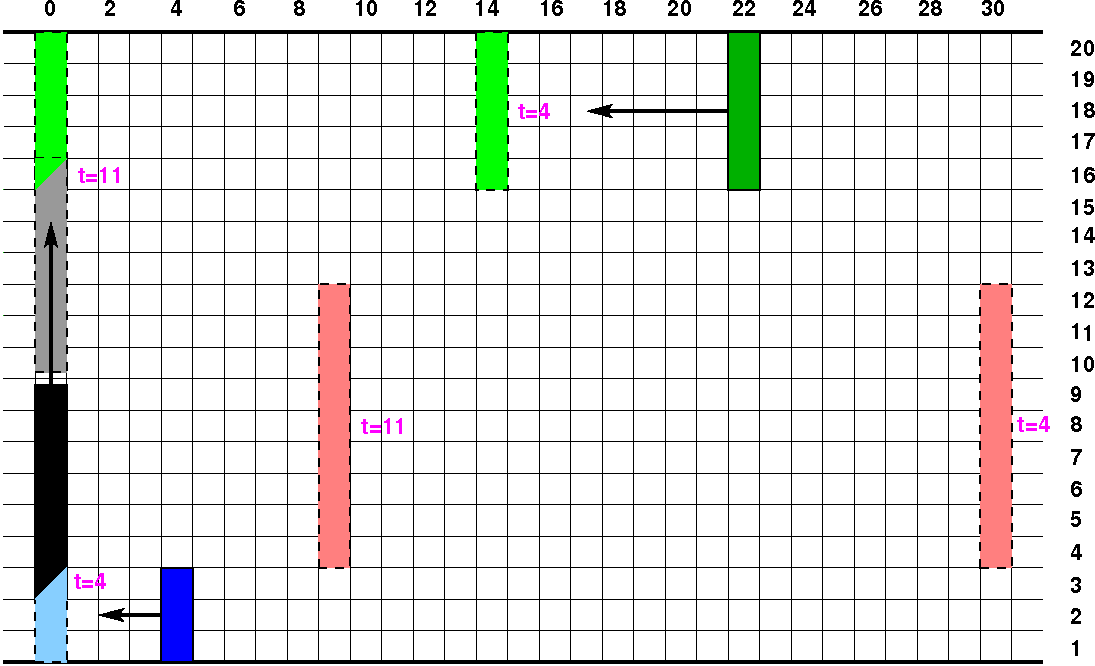
\includegraphics[width=0.75\textwidth]{fiskspelet2.png}\\
\caption{Situationen i exempelfall 2}
\label{fig:sample2}
\end{figure}
En möjlig lösning till det andra exemplet visas i figur~\ref{fig:sample2}.
Den svarta rektangeln visar var du måste befinna dig vid tiden $t=4$ sekunder när du äter den blå
lilla fisken (det går bra att även ha detta som utgångsposition). Den
delade rutan markerar att fiskarna överlappar på denna ruta. Sedan
måste du röra dig i full fart uppåt för att kunna äta den gröna
mellanfisken vid $t=11$ (din position visas då av den grå streckade
rektangeln). Slutligen måste du fortsätta uppåt för att undkomma den
röda stora fisken som når din kolumn vid $t=14$ (detta skulle bli för
kladdigt att visa i figuren).